% time values for run2, run6 and run7
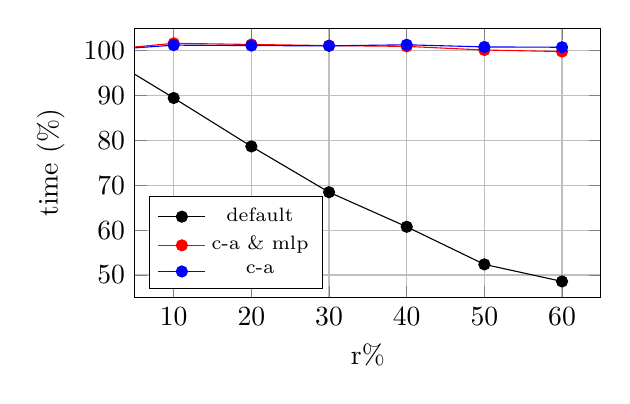
\begin{tikzpicture}
\begin{axis}[
    title={},
    height=5cm,
    width=7.5cm,
    xlabel={r\%},
    ylabel={time (\%)},
    xmin=5, xmax=65,
    ymin=45, ymax=105,
    xtick={10,20,30,40,50,60},
    ytick={40,50,60,70,80,90,100},
    legend pos=south west,
    xmajorgrids=true,
    ymajorgrids=true,
    legend style={font=\scriptsize}
]

\addplot[
    color=black,
    mark=*
    ]
    coordinates {
    (0,100)(10,89.45)(20,78.65)(30,68.45)(40,60.74)(50,52.36)(60,48.56)
    };
    
\addplot[
    color=red,
    mark=*
    ]
    coordinates {
    (0,100)(10,101.64)(20,101.38)(30,101.13)(40,100.95)(50,100.14)(60,99.80)
    };

\addplot[
    color=blue,
    mark=*
    ]
    coordinates {
    (0,100)(10,101.23)(20,101.13)(30,101.07)(40,101.31)(50,100.83)(60,100.76)
    };
    
\legend{default, c-a \& mlp, c-a}
    
\end{axis}
\end{tikzpicture}